\documentclass[a0,final, portrait]{inriaposter}

\usepackage[utf8]{inputenc}
\usepackage[OT1]{fontenc}
\usepackage[english]{babel}
\usepackage{amsfonts, amsmath, amssymb, amsthm, dsfont, amsthm}
\usepackage{paralist}
\usepackage{wrapfig}

\usepackage{caption}
\usepackage{subcaption} 

\usepackage{graphics}
\usepackage{graphicx}

\usepackage{epstopdf}

\providecommand{\mtx}[1]{\mathbf{#1}}

\begin{document}

\sffamily

\postertitle%
{Calibration-Free BCI Based Control}
{Jonathan Grizou \textsuperscript{1} \; and \; Iñaki Iturrate\textsuperscript{2} \; and \\ Luis Montesano\textsuperscript{3} \; and \; Pierre-Yves Oudeyer\textsuperscript{1} \; and \; Manuel Lopes\textsuperscript{1}}{\Large  \textsuperscript{1} Flowers Team,  INRIA / ENSTA ParisTech, France \; --- \; \textsuperscript{2} CNBI, EPFL, Switzerland \; --- \; \textsuperscript{3} I3A, University of Zaragoza, Spain}

\vfill
%\vspace{1cm}
\begin{multicols}{2}
\Large

\blockabstract{
\textbf{Can a system learn a task from human instructions if it does not known how to interpret the human communicative signals?} In the machine learning literature, agents have access to known sources of information (rewards, correct demonstrations, symbolic instructions). Part of the work done in Human Machine Interaction consists of translating human signals (speech, gestures, EEG, \ldots) to symbolic instructions usable by the system. Such signal to meaning mapping requires to train a specific classifier for each user. Training this classifier is time consuming and requires an expert to tune the parameters and collect signal samples. 
\medskip
\par {~~~~~}The idea behind this work is to create calibration free systems that can learn a signal to meaning mapping while learning the task taught by the user. Consider for example the case of a Brain Computer Interaction system that would not require the fastidious calibration procedure.
}

\block{Motivation}{
\vspace{-1cm}
\begin{center}
	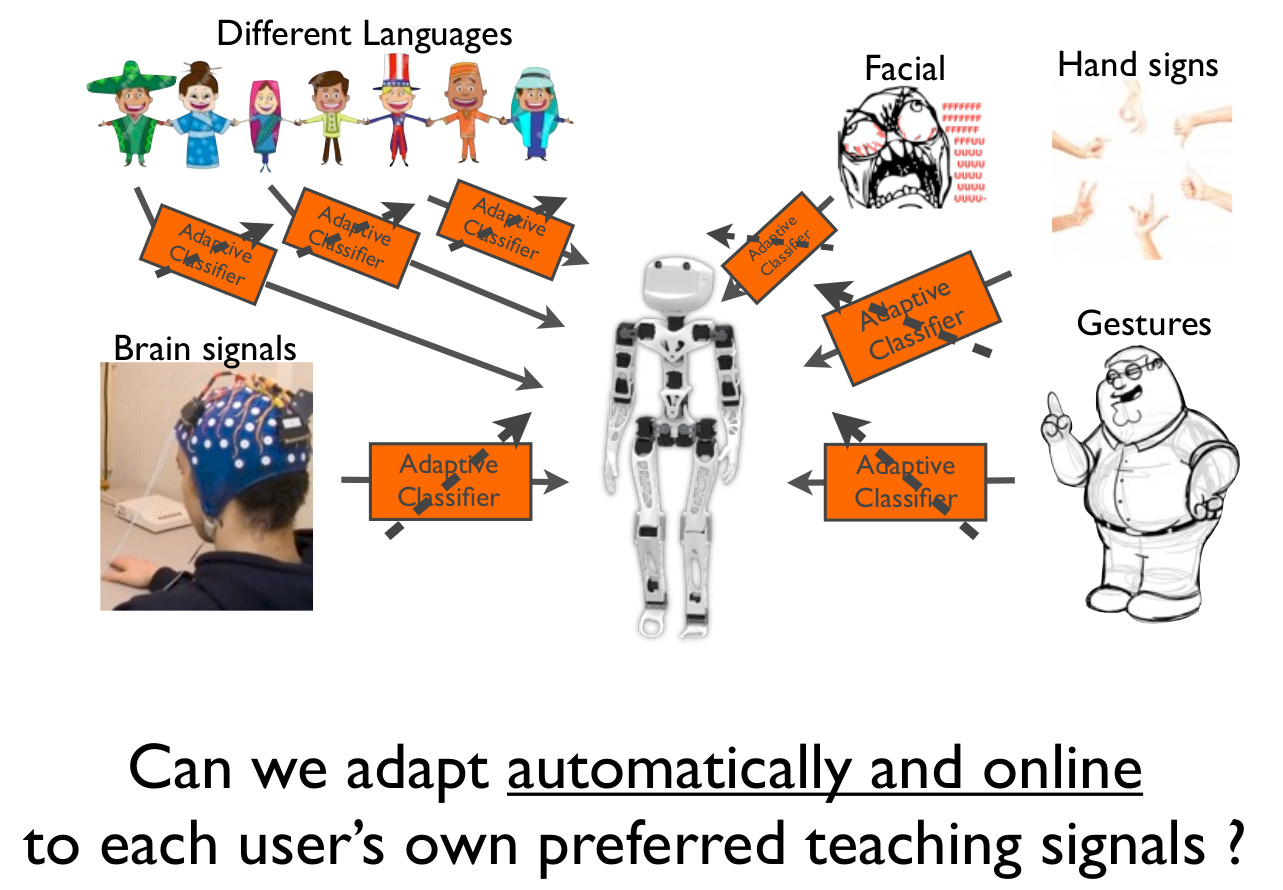
\includegraphics[width=0.7\columnwidth, trim=0cm 8cm 0cm 0cm, clip=true]{images/question.png}

	\LARGE{Can we adpat \textbf{automatically and online} \\ to each user's own preferred teaching signals ?}
\end{center}
}

\block{Problem}{
\vspace{-1cm}
\begin{center}
	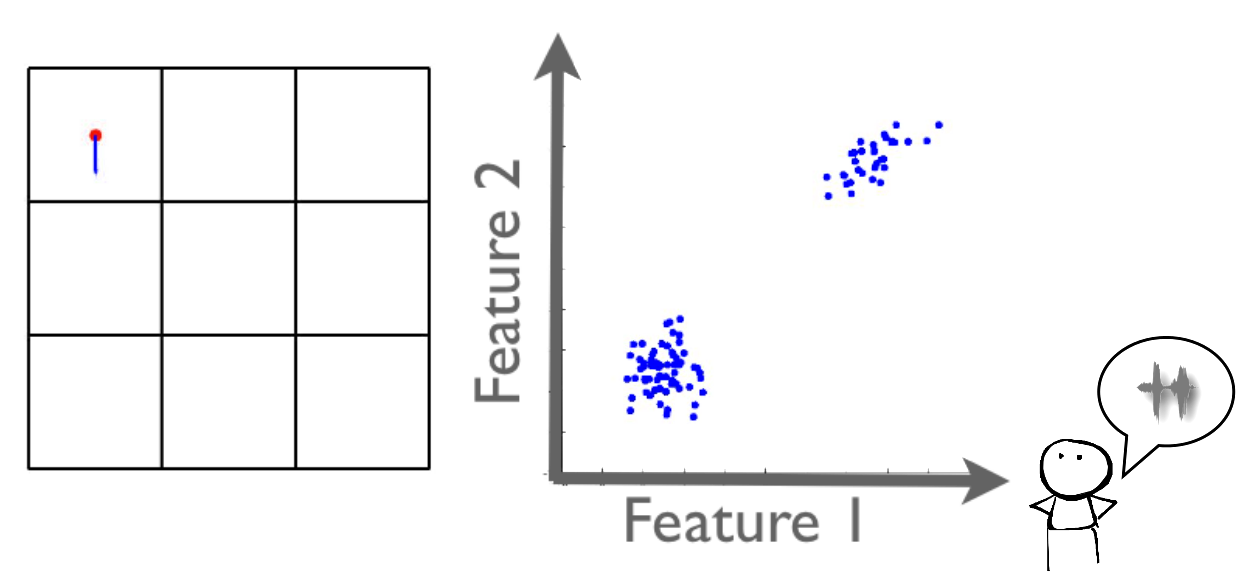
\includegraphics[width=0.7\columnwidth, trim=0cm 0cm 8cm 0cm, clip=true]{images/exemple.png}
\end{center}
}

\block{How it works}{

For successful communication the human and the robot need to share a common background. Usually it is the meaning of the instructions or demonstrations. We exploits task constraints to build a distribution of possible tasks, and generate interpretation hypothesis of the EEG signals according to each hypothetic task. 

\begin{center}
\begin{minipage}{.46\columnwidth}
	\begin{center}
		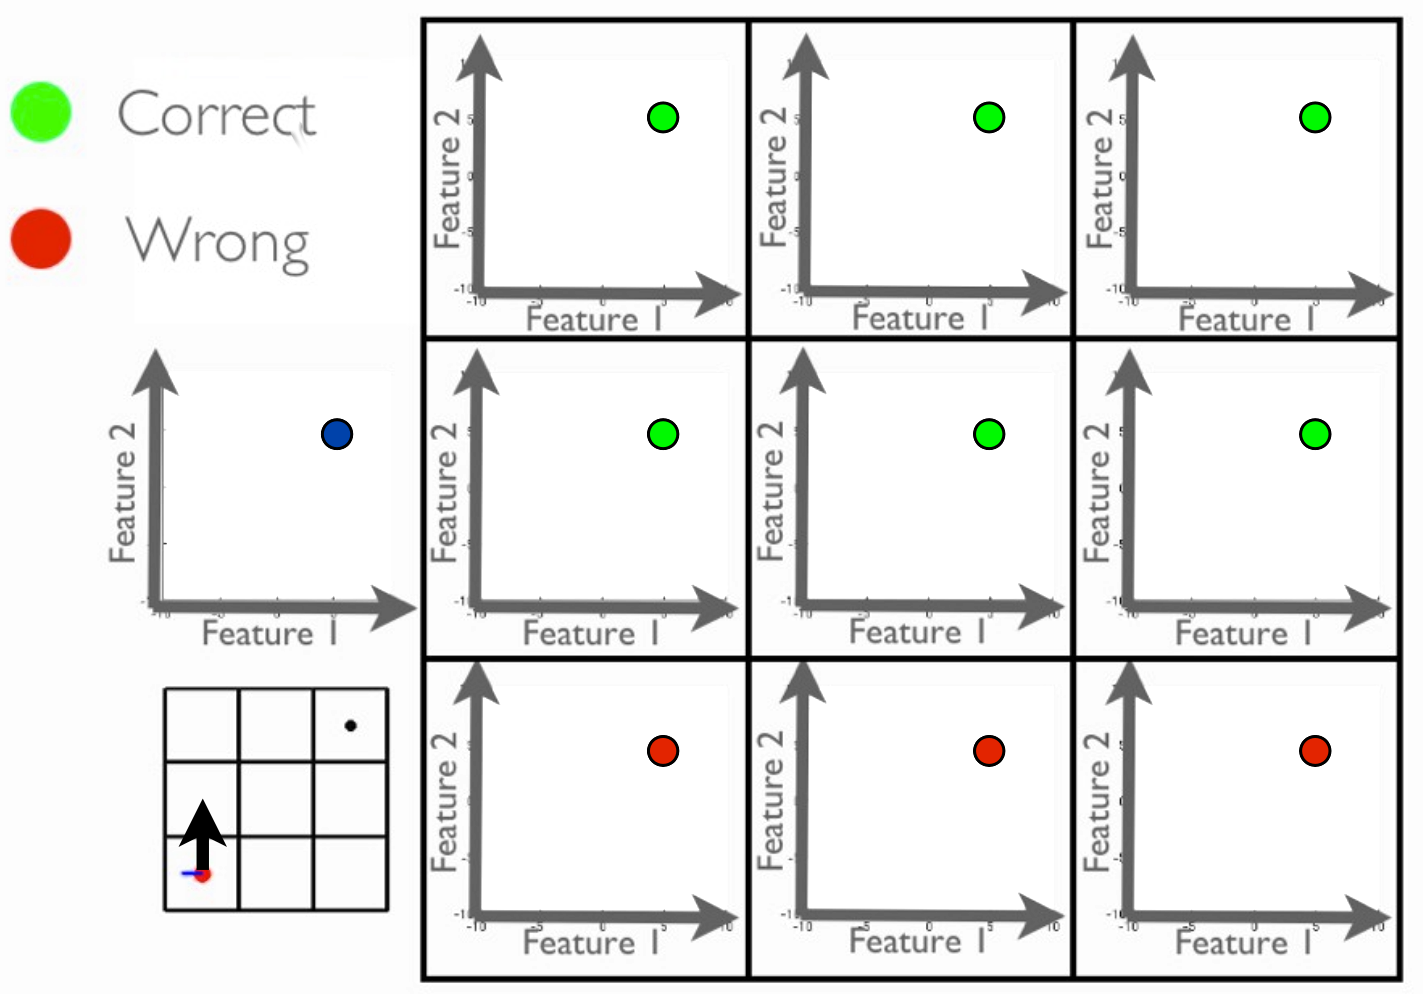
\includegraphics[width=\columnwidth]{images/toy_solution.png}
	\end{center}
\end{minipage}
\begin{minipage}{.02\columnwidth}
	\begin{center}

	\end{center}
\end{minipage}
\begin{minipage}{.442\columnwidth}
	\begin{center}
		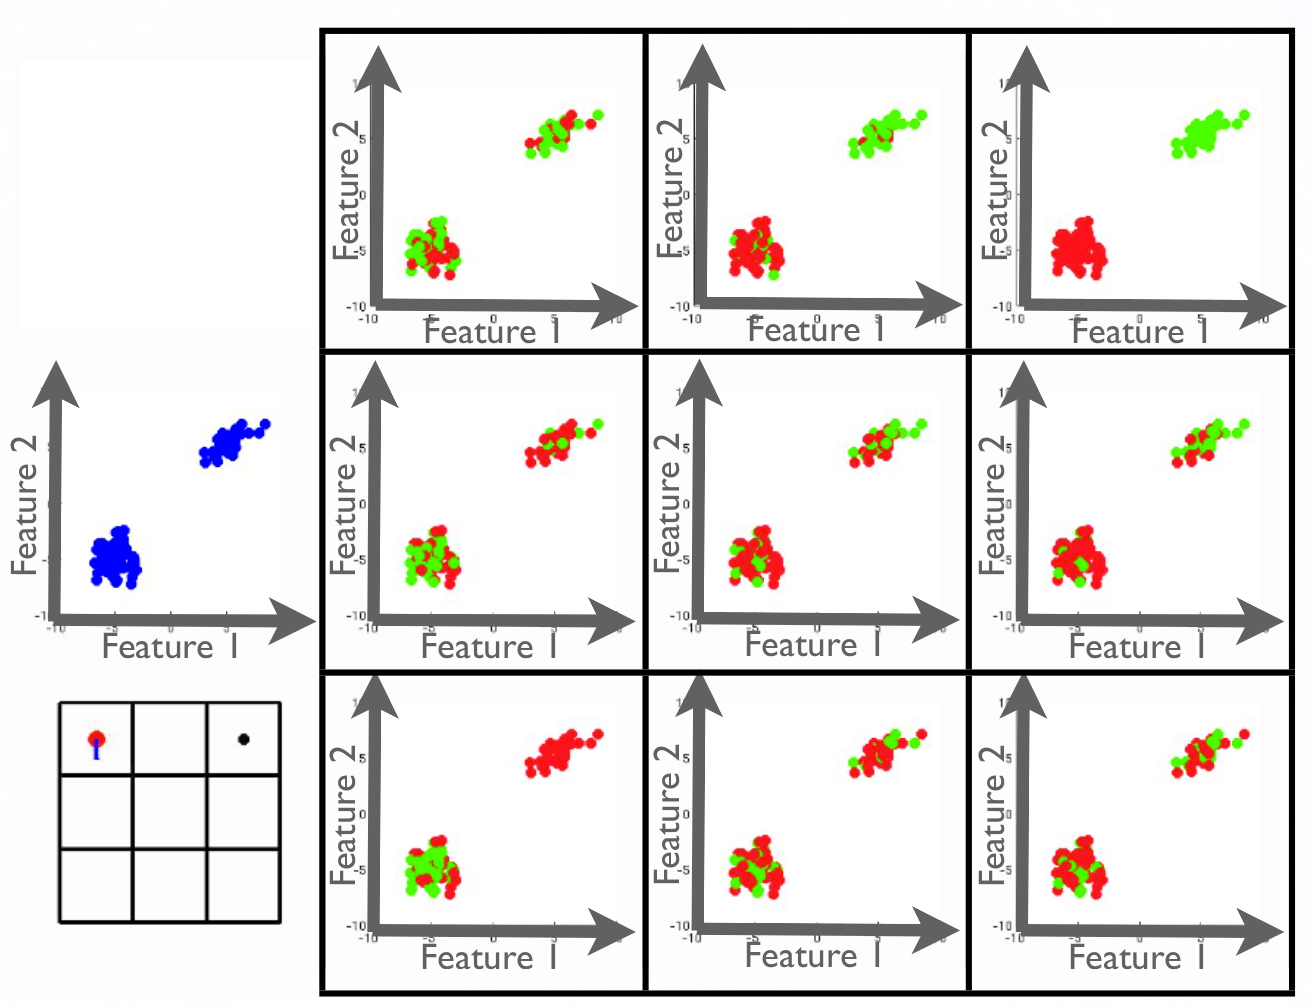
\includegraphics[width=\columnwidth]{images/toy_sol.png}
	\end{center}
\end{minipage}
\end{center}

We select the hypothesis which best explains the history of interaction. Since the correct task will assign the correct labels to the signals, and the wrong task will assign some wrong labels, the expected classification rate is a good measure to identify the task intended by the user.

}

\block{Results}{

\begin{center}
{\LARGE \textbf{BCI Control with Human Subjects}}
\end{center}

\vspace{1cm}

We report experiments where four users use BCI to control an agent on a virtual world to reach a target without any previous calibration process.

\vspace{1cm}

\begin{center}
\begin{minipage}{.46\columnwidth}
\begin{center}
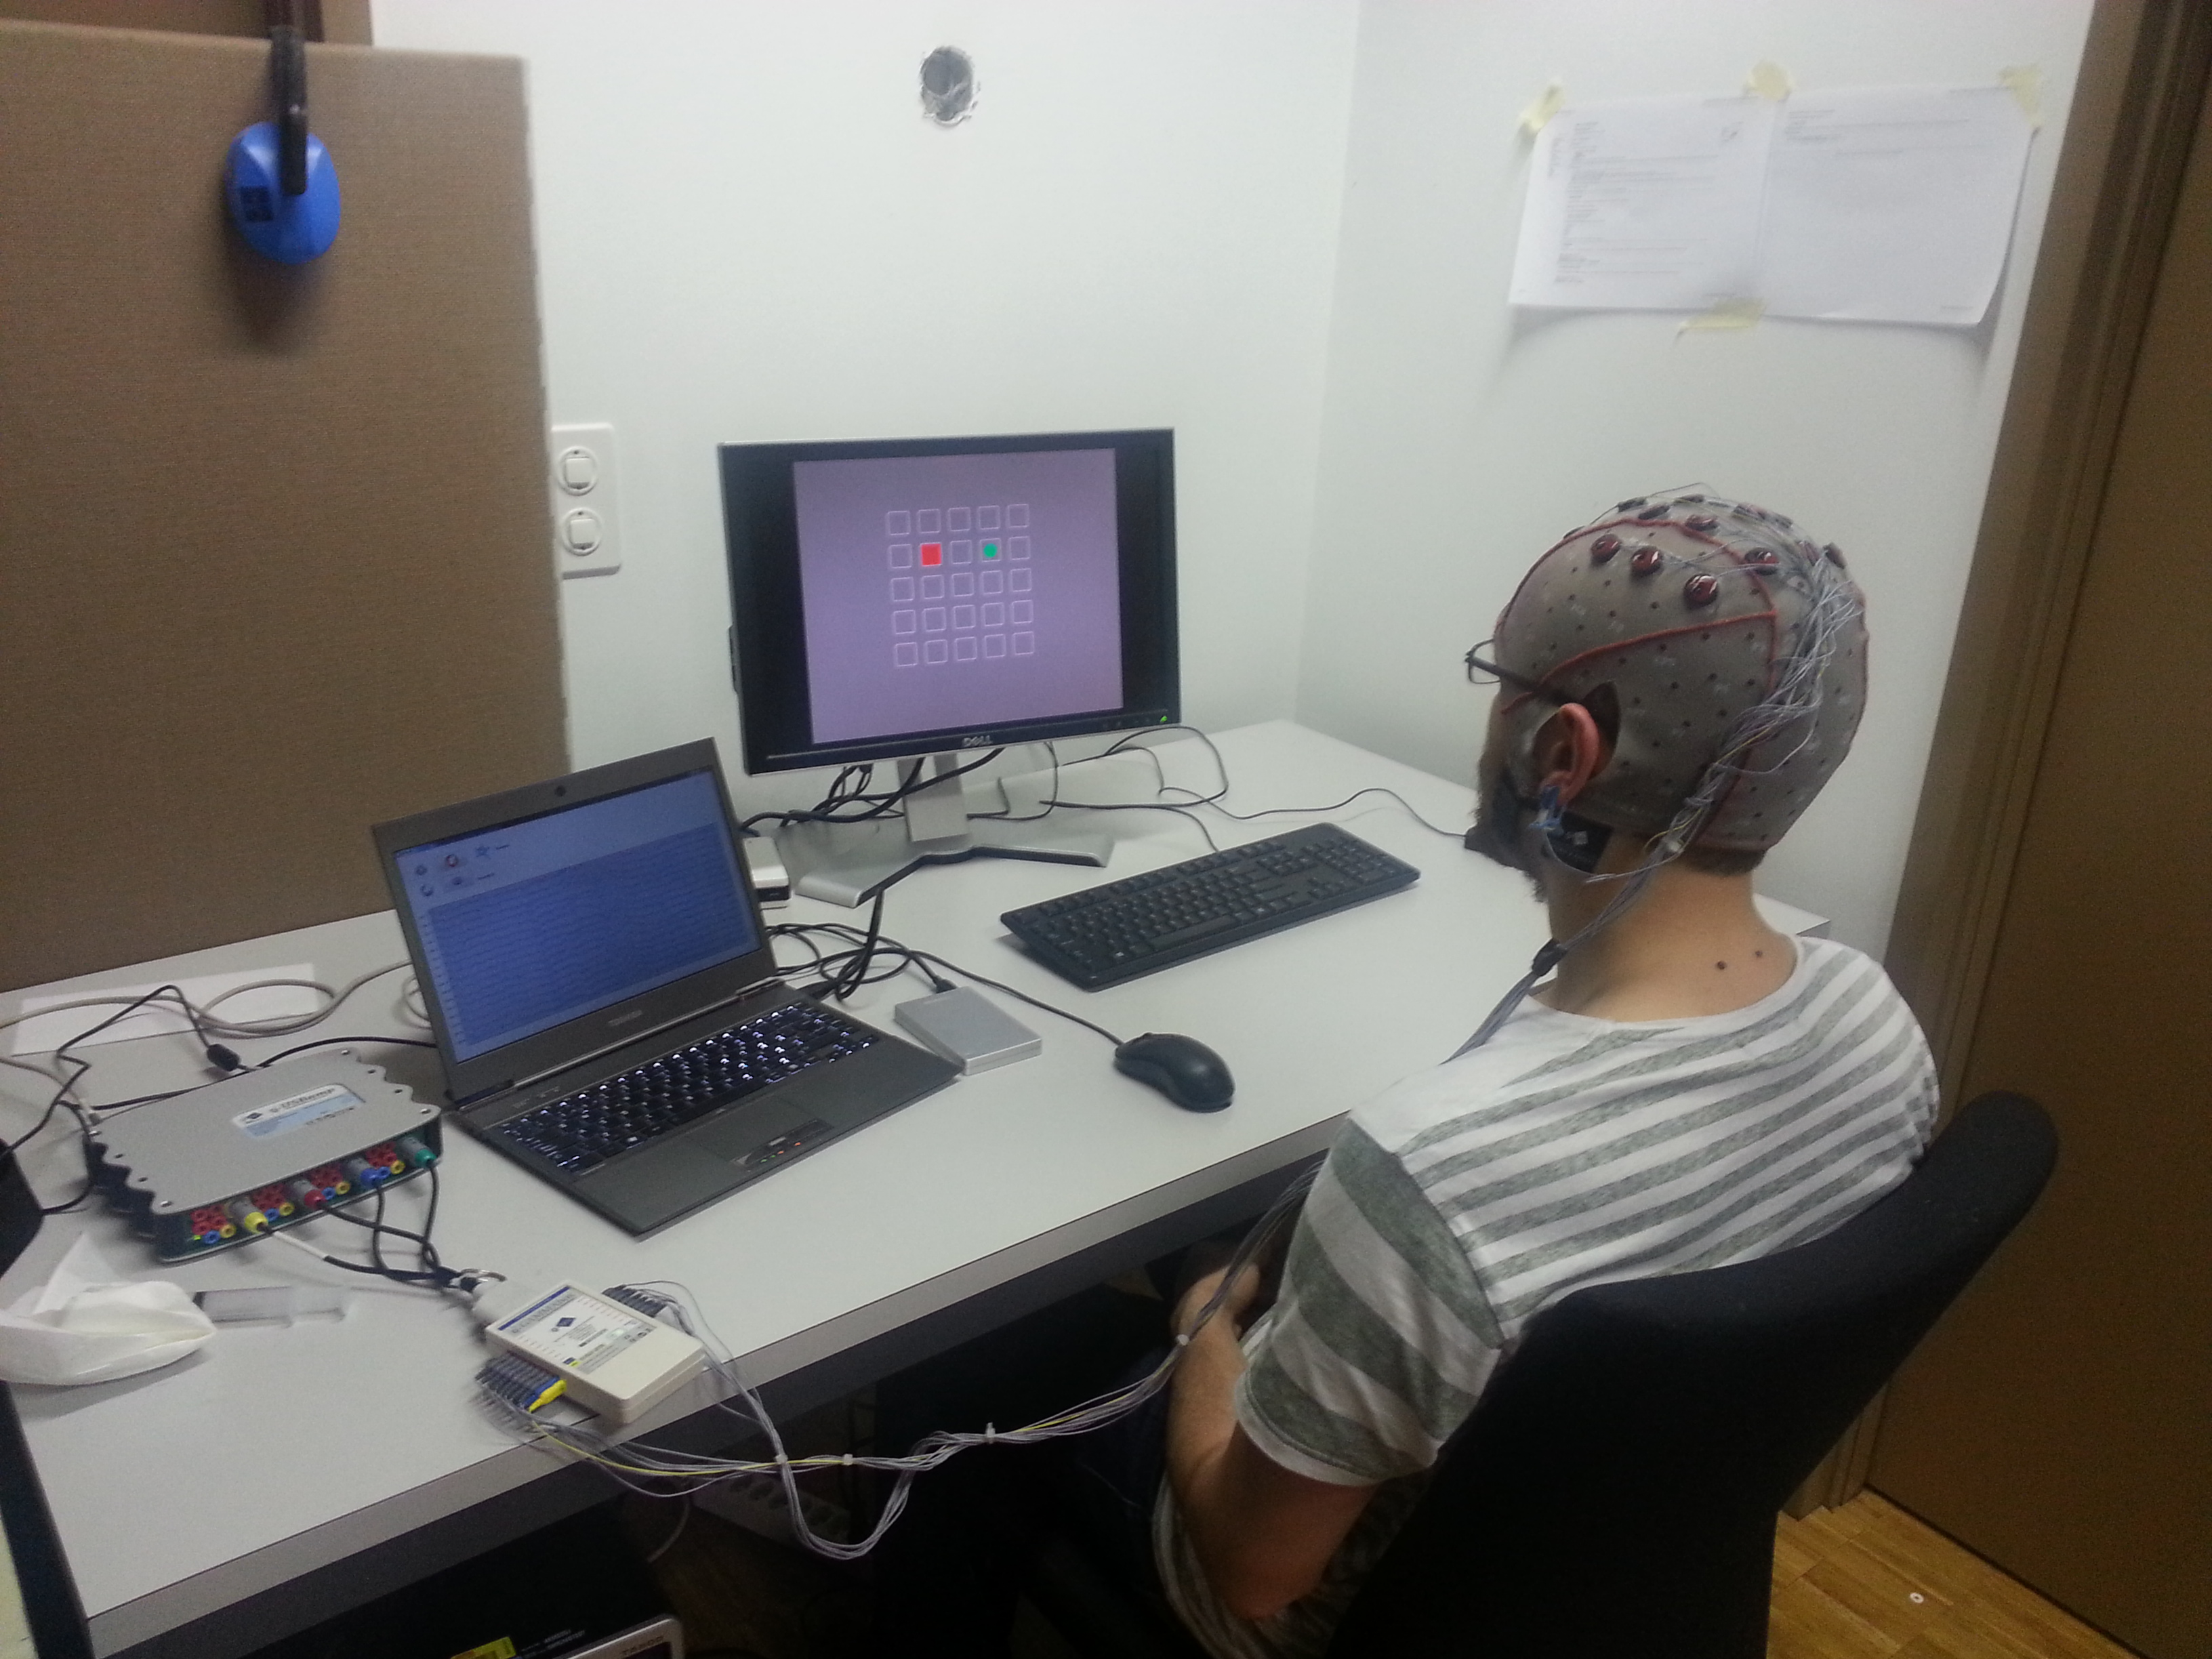
\includegraphics[width=\columnwidth, trim=2cm 10cm 10cm 15cm, clip=true]{images/BCI_setup2.jpg}
\end{center}
\end{minipage}
\begin{minipage}{.02\columnwidth}
	\begin{center}

	\end{center}
\end{minipage}
\begin{minipage}{.46\columnwidth}
\begin{center}
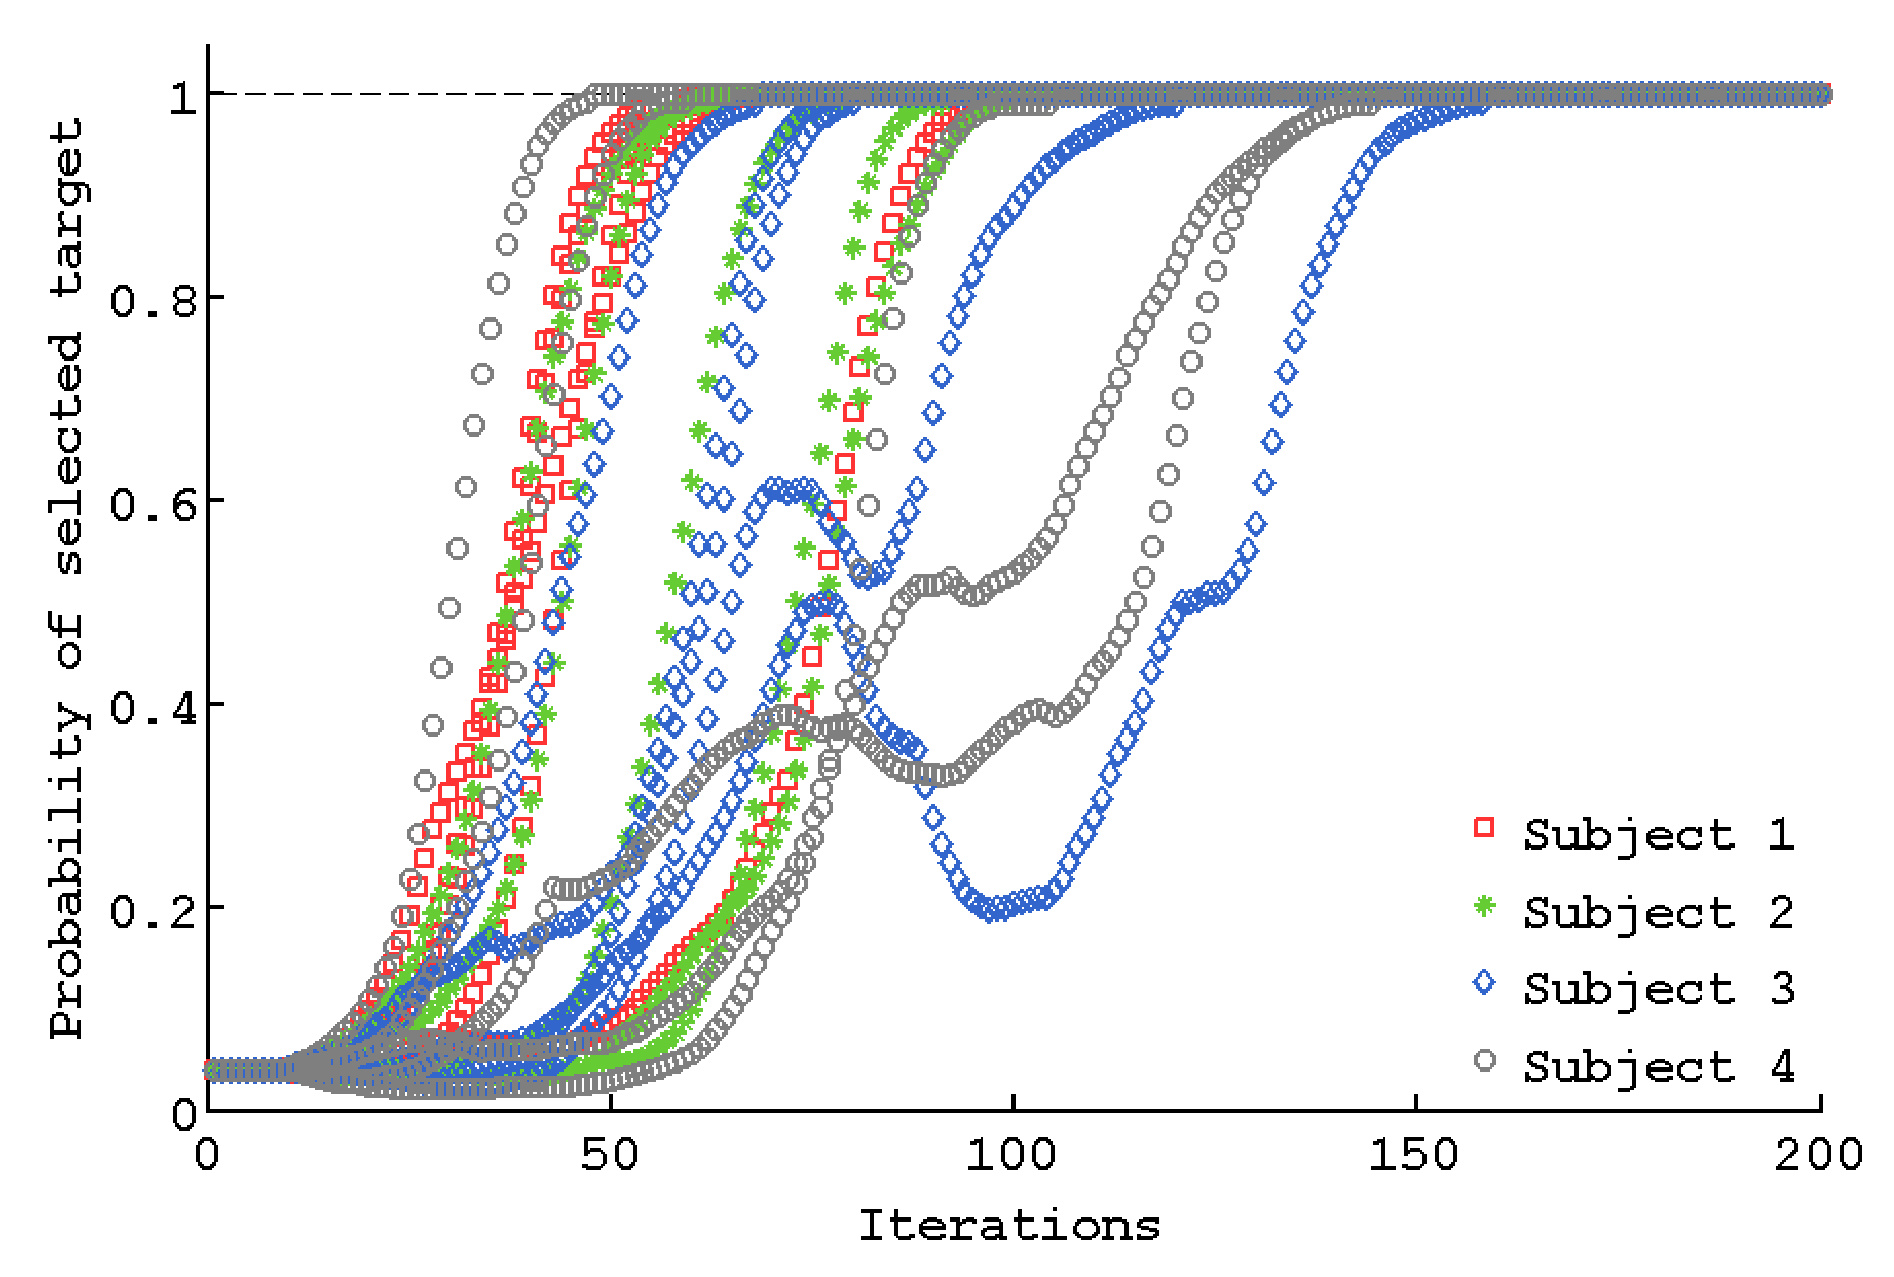
\includegraphics[width=\columnwidth]{images/plot_realevolution}	
\end{center}
\end{minipage}
\end{center}

\vspace{1cm}

We introduce a measure of uncertainty on the task and on the EEG signals interpretation to act as an exploratory bonus for a planning strategy. This speeds up learning by guiding the system to regions that better disambiguate among task hypotheses. 

\vspace{1cm}

\begin{center}
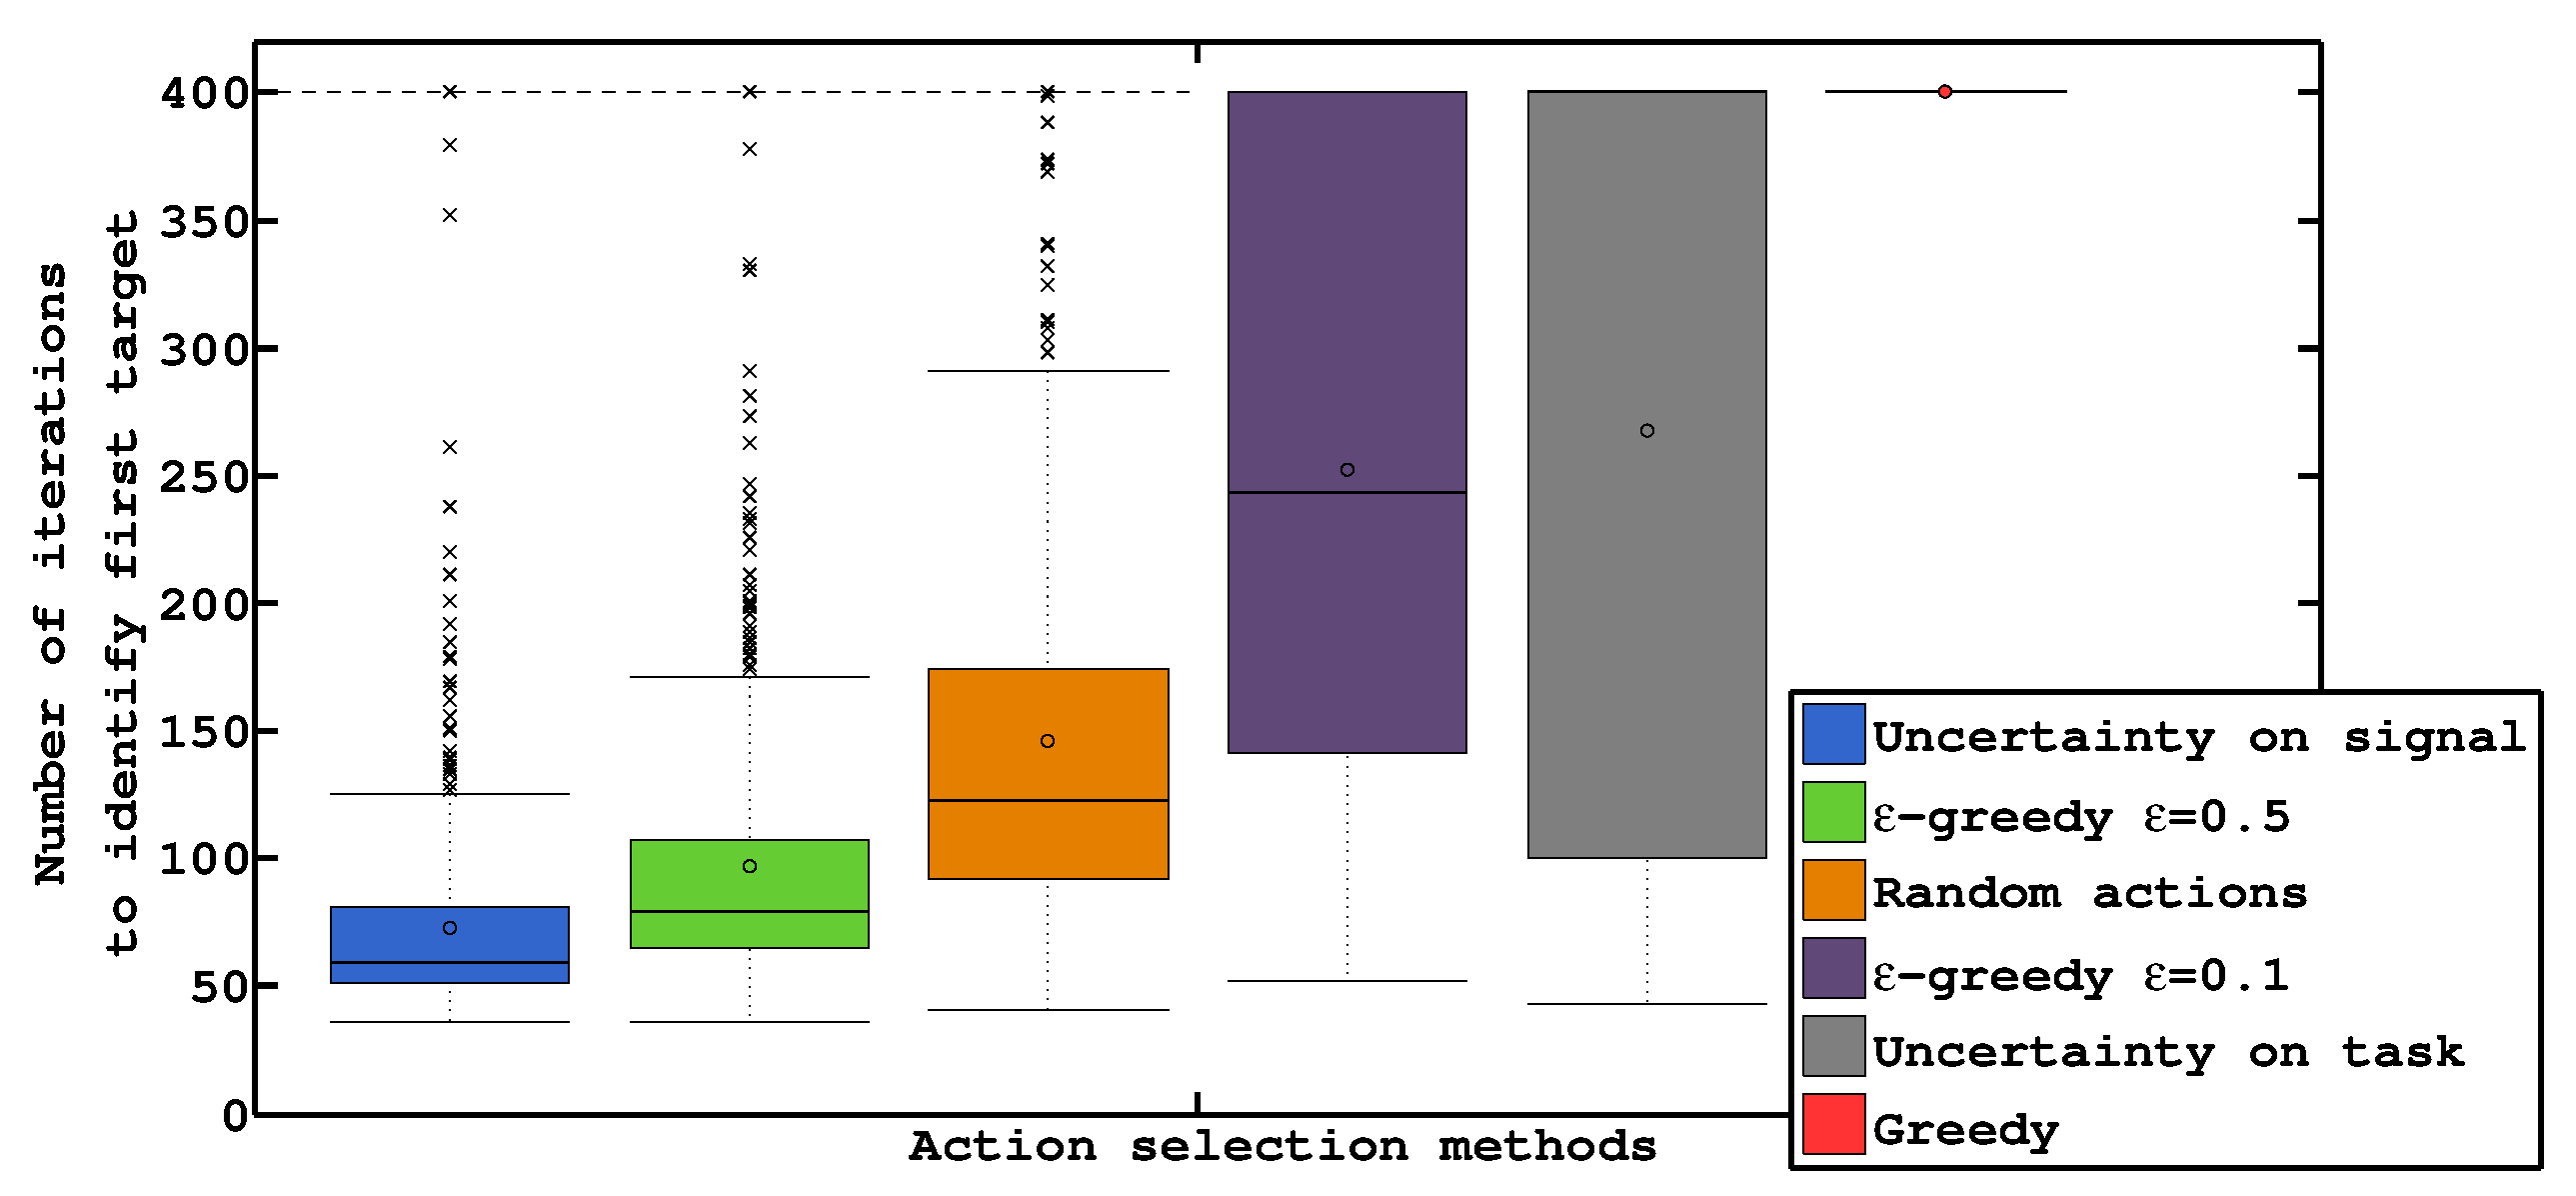
\includegraphics[width=0.85\columnwidth]{images/plot_planning_first}
\end{center}

\vspace{1cm}

We show that we can identify an average of 20 tasks in 400 iterations for EEG dataset of reasonably good quality. Furthermore the system identifyied correctly most of the labels associated with the EEG signals.

\vspace{1cm}

\begin{center}
\begin{minipage}{.46\columnwidth}
\begin{center}
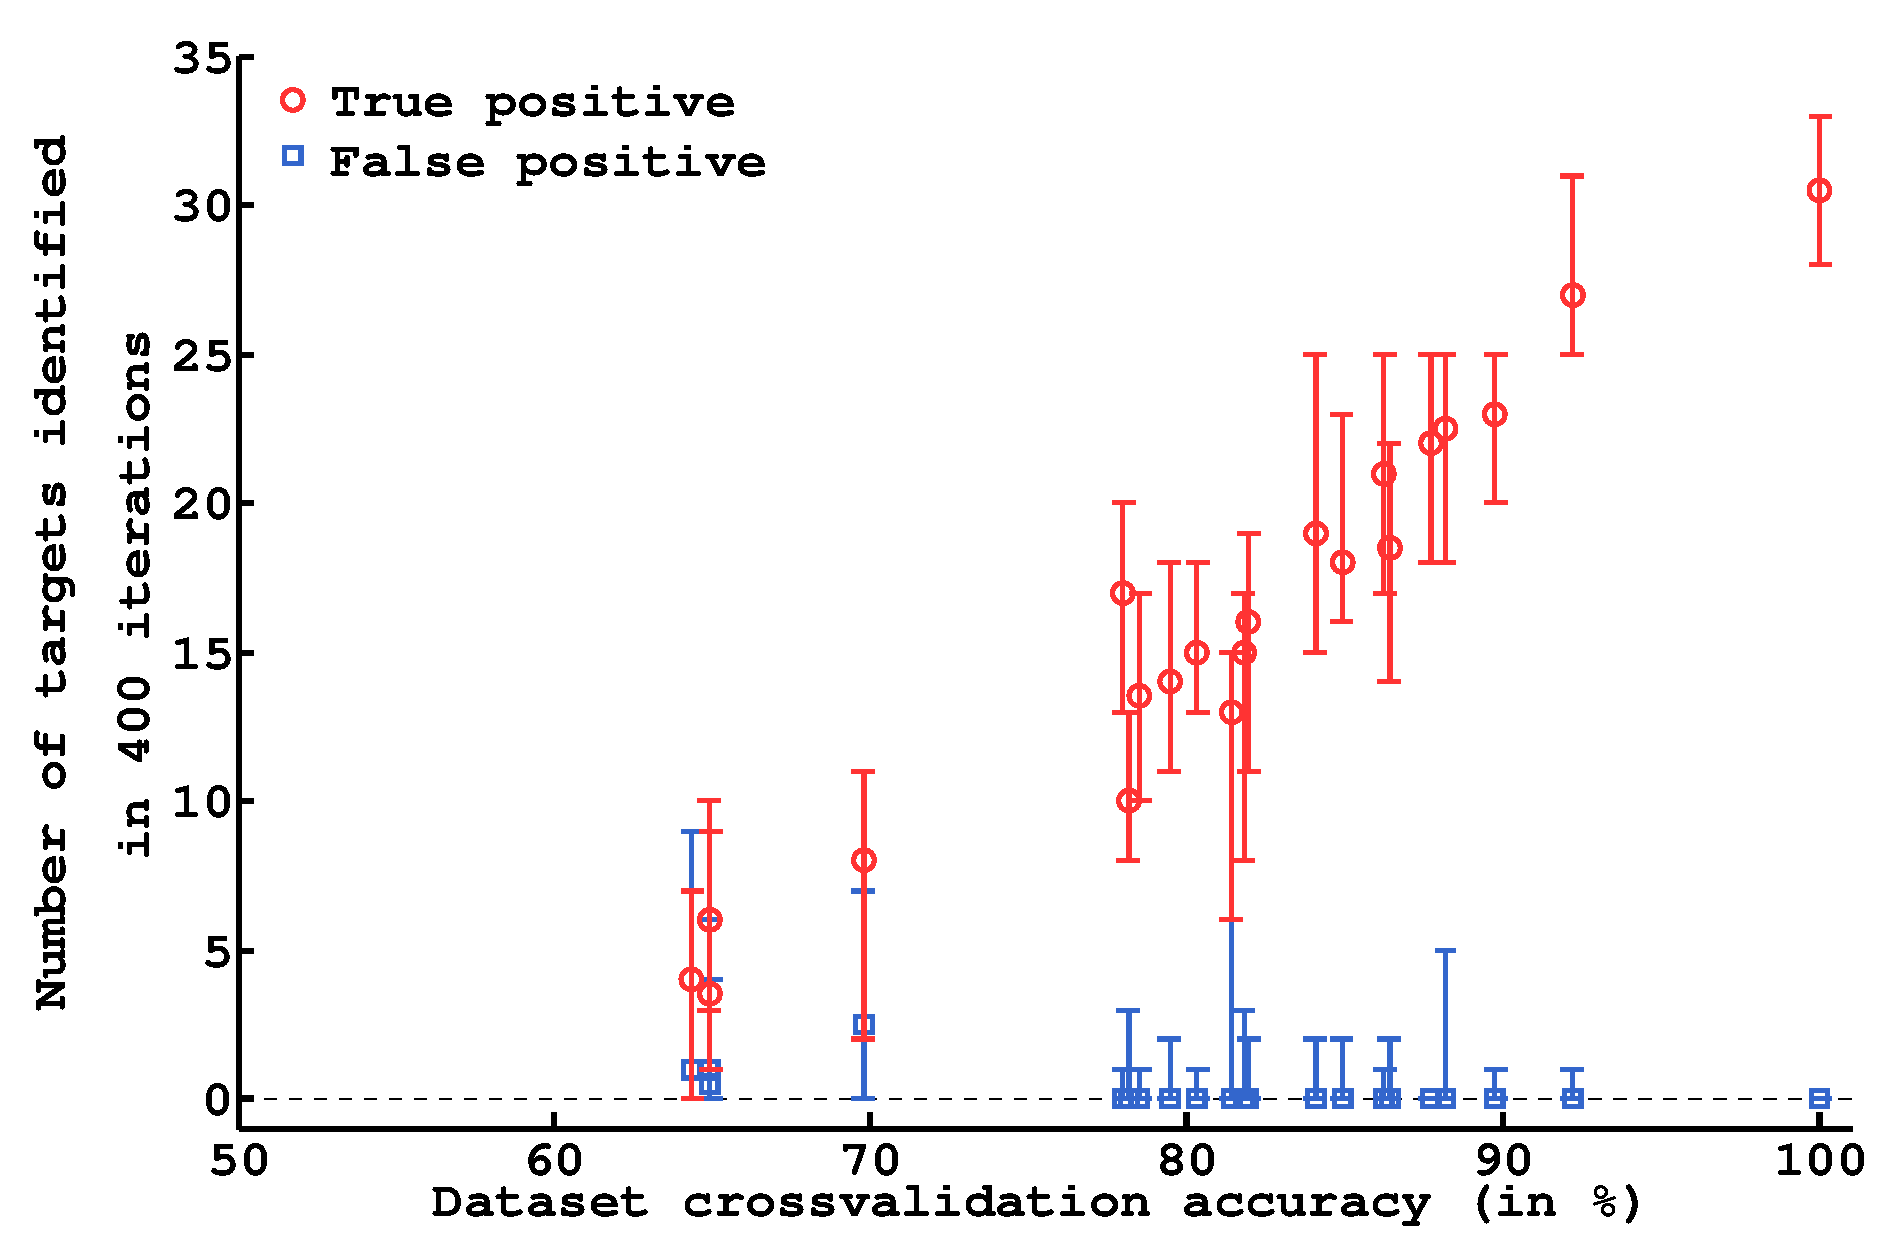
\includegraphics[width=\columnwidth]{images/plot_first400_reach}
\end{center}
\end{minipage}
\begin{minipage}{.02\columnwidth}
	\begin{center}

	\end{center}
\end{minipage}
\begin{minipage}{.46\columnwidth}
\begin{center}
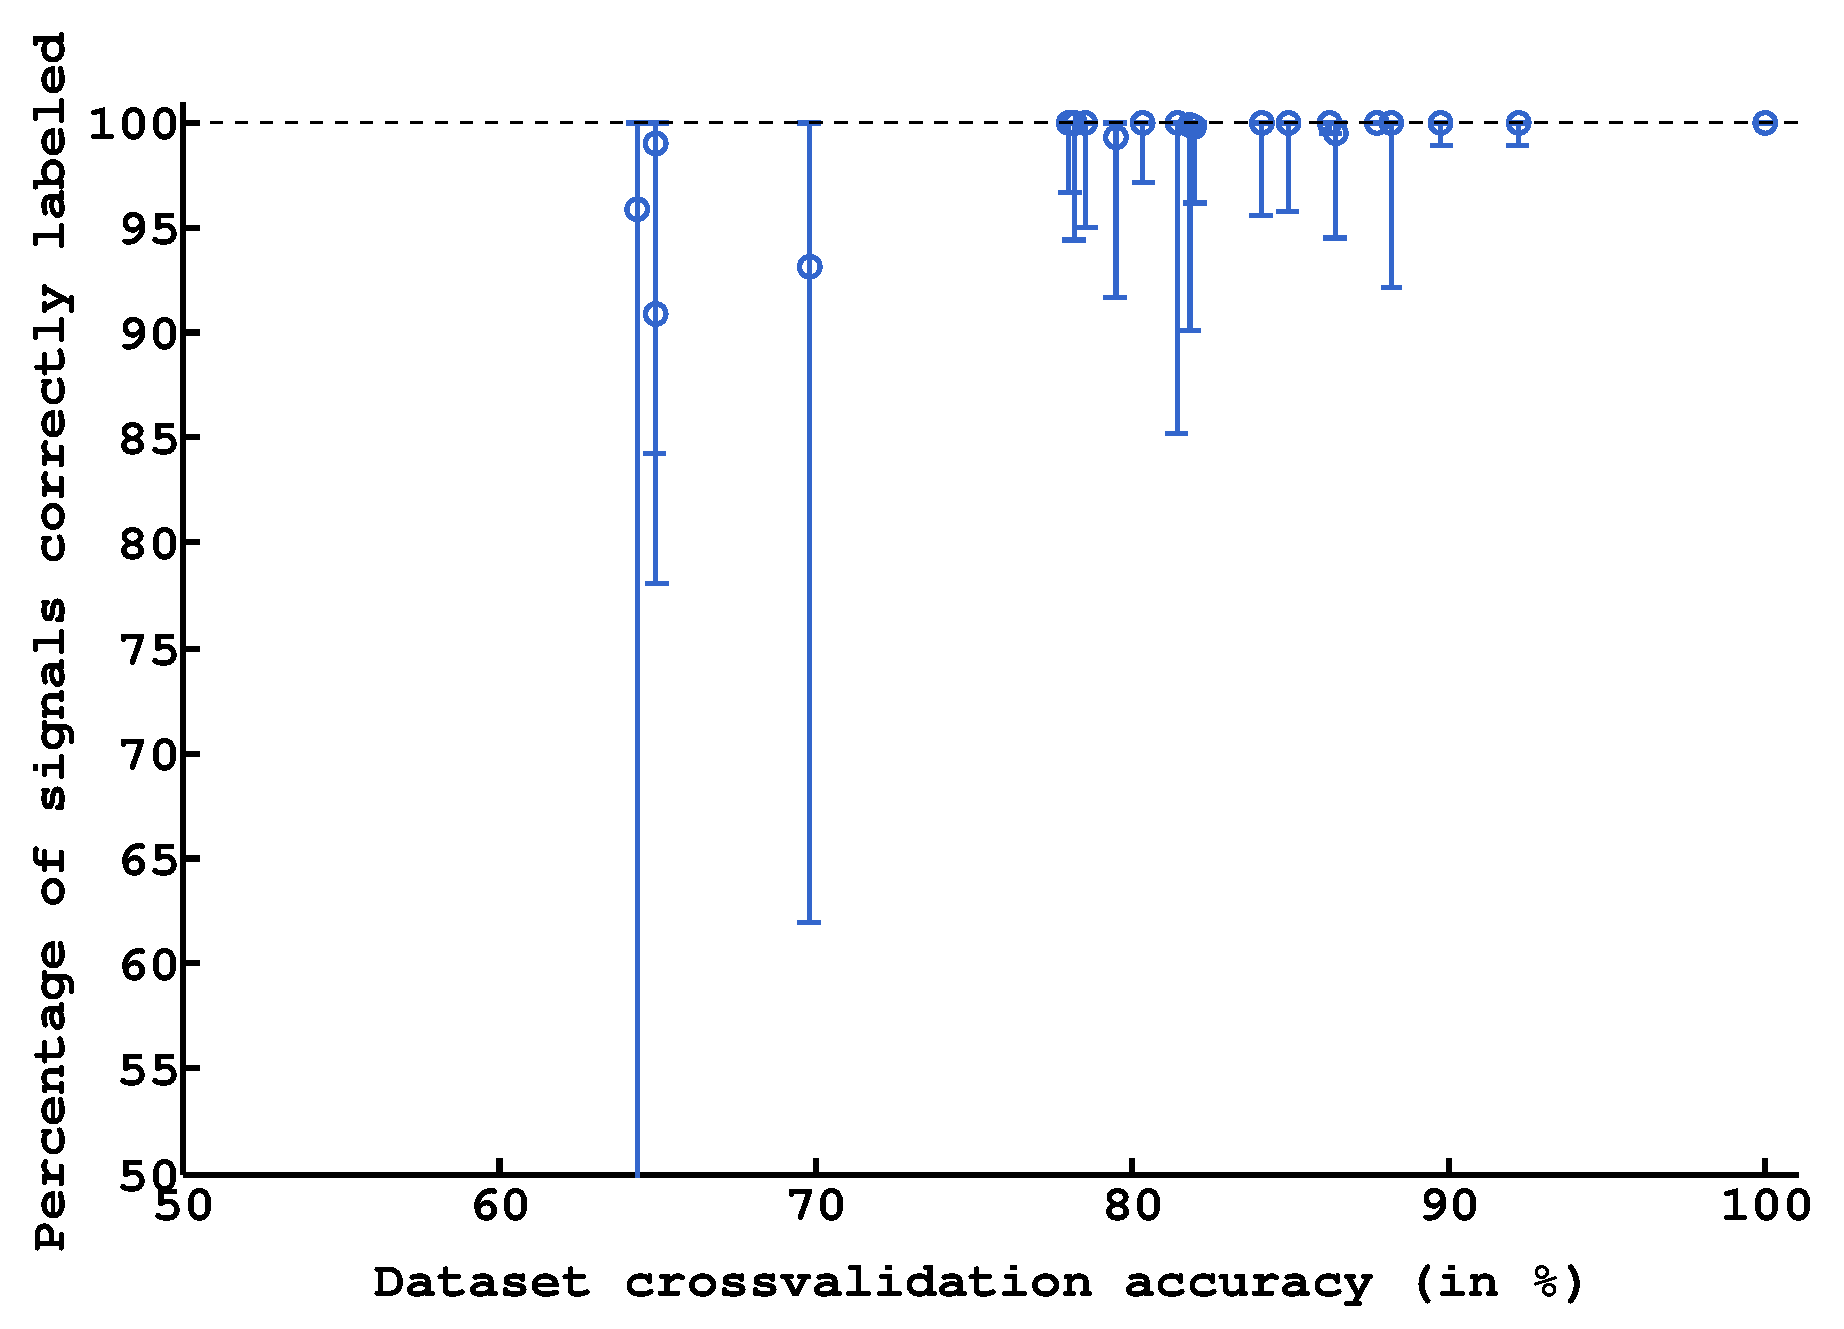
\includegraphics[width=\columnwidth]{images/plot_percent_label}	
\end{center}
\end{minipage}
\end{center}

}


\block{Conclusion}
{
\textbf{Proposed algorithm:}
\begin{inparaenum}
\item Learns a task from unlabeled and noisy instructions.
\item Reuses acquired knowledge.
\item Makes use of uncertainty on the signal and task space to improve learning performances.
\end{inparaenum}

\textbf{Of interest:}
\begin{inparaenum}
\item Signals expressed as feature vectors, which can encode facial expression, gesture, speech, EEG, \ldots
\item Works with any classification algorithm.
\end{inparaenum}
}

\block{References}
{
	% \vspace{-10pt}
	\nocite{*}
	\bibliographystyle{abbrv}
	\renewcommand{\section}[2]{}% Hack to remove bibliography title
	\bibliography{ref}
	\vspace{-10pt}
}

\end{multicols}
\vfill
\end{document}
